\section{Experiment Design and Results}

\subsection{Experiment Design}

Since our project was focused on the NN-based agents, we set up our experiments to test its performance as we trained it in the following way.
The \texttt{nnAgent} being tested, call it \texttt{ourHero}, will train against a \texttt{SearchAgent} as a sparring partner for a specified number of games.
Then, we perform a test, which corresponds to \texttt{ourHero} facing each opponent in a gauntlet in a specified number of games, with output reported.
(Note that we do not halt weight updates during testing, so we have a slight distinction from the traditional train/test separation).
As this process is repeated for a large number of testing sessions, we report win/loss/draw count, \# of illegal moves, maximum game length (in moves) and average game length (also in moves).
Note that since we executed all this code on CPUs, not GPUs, our network is not very deep since we could not devote a great deal of compute to training.
Similarly, the \texttt{SearchAgent} does very few rollouts -- merely 5 (as we achieve better performance we can add agents which perform more accurate value estimation to the gauntlet).


\subsection{Results}
We wanted to sample from the amount of time that the agent had had to train before going into the gauntlet.
We hypothesized that the more time that the agent had had to train before entering, the better that it would perform against the opposing agents.
However, we were surprised to learn that the agent performed \emph{decreasingly} better as the amount of training games increased.
\begin{table}
\begin{tabular}{@{}p{.18\columnwidth}|p{.4\columnwidth}|p{.33\columnwidth}}
\hline
Training Games & Random Agent (Win\%) & Bad Search(Win\%)\\
\hline
50 & 83 & 13 \\
\hline
100 & 74 & 15\\
\hline
150 & 75 & 13\\
\hline
200 & 69 & 16\\
\end{tabular}
\vspace{2pt}
\caption{ Using the Adam optimizer, we used a learning rate of 1e-3 and a weight decay of 1e-4 to obtain these results. The total number of games tested was 100, so the percentages (the right two columns) were computed by $(numWins/numGames)\times 100$ }
\label{tab:results}
\end{table}

%\begin{figure}[b]
	\centering
	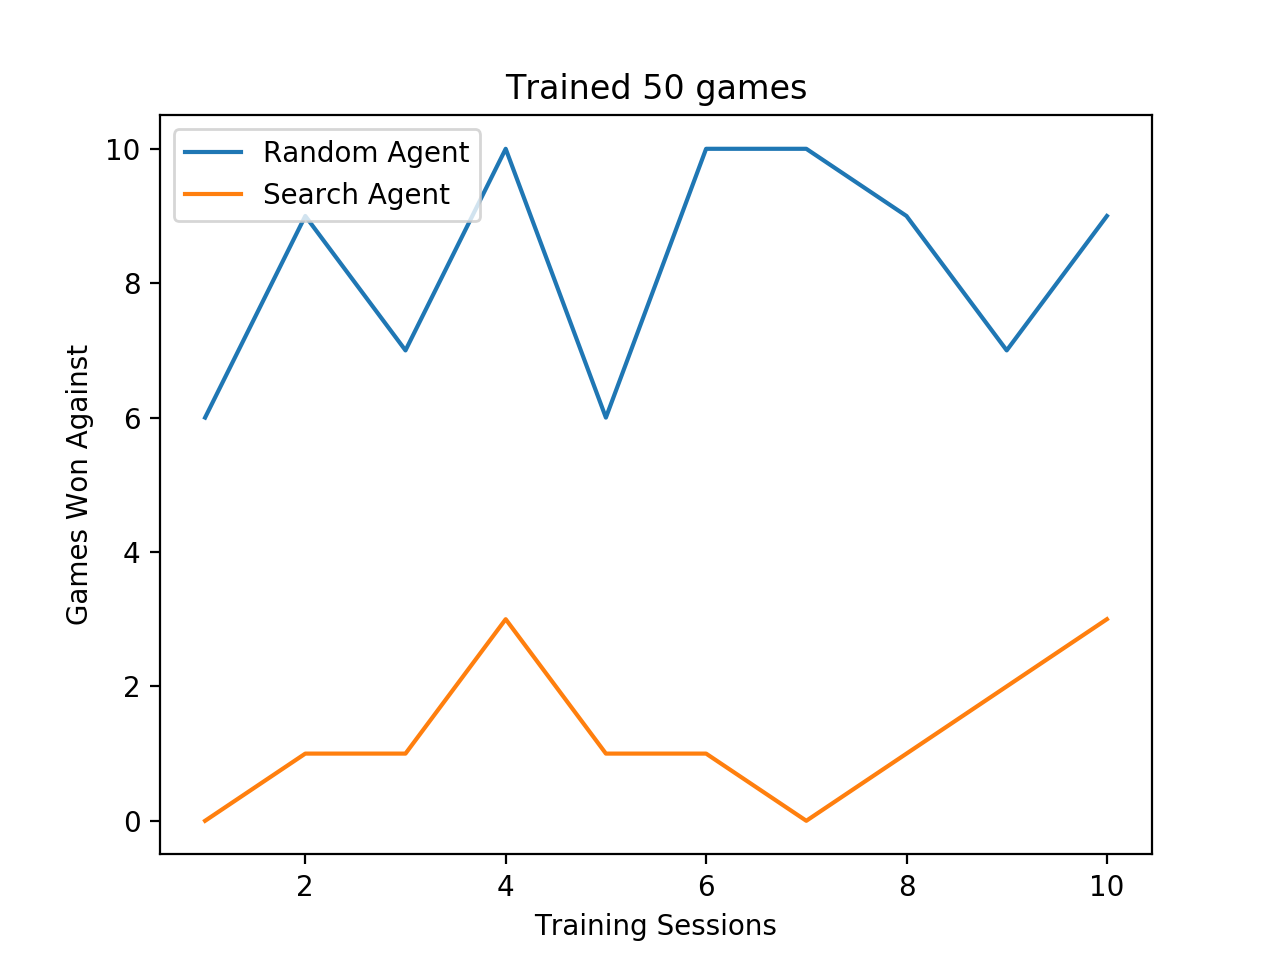
\includegraphics[ width = \columnwidth ]{Assets/50TrainedGames}
	\caption{Our results from when the sampling occurs after 50 training sessions}
	\label{fig:50TrainResults}
\end{figure}
\begin{figure}[b]
	\centering
	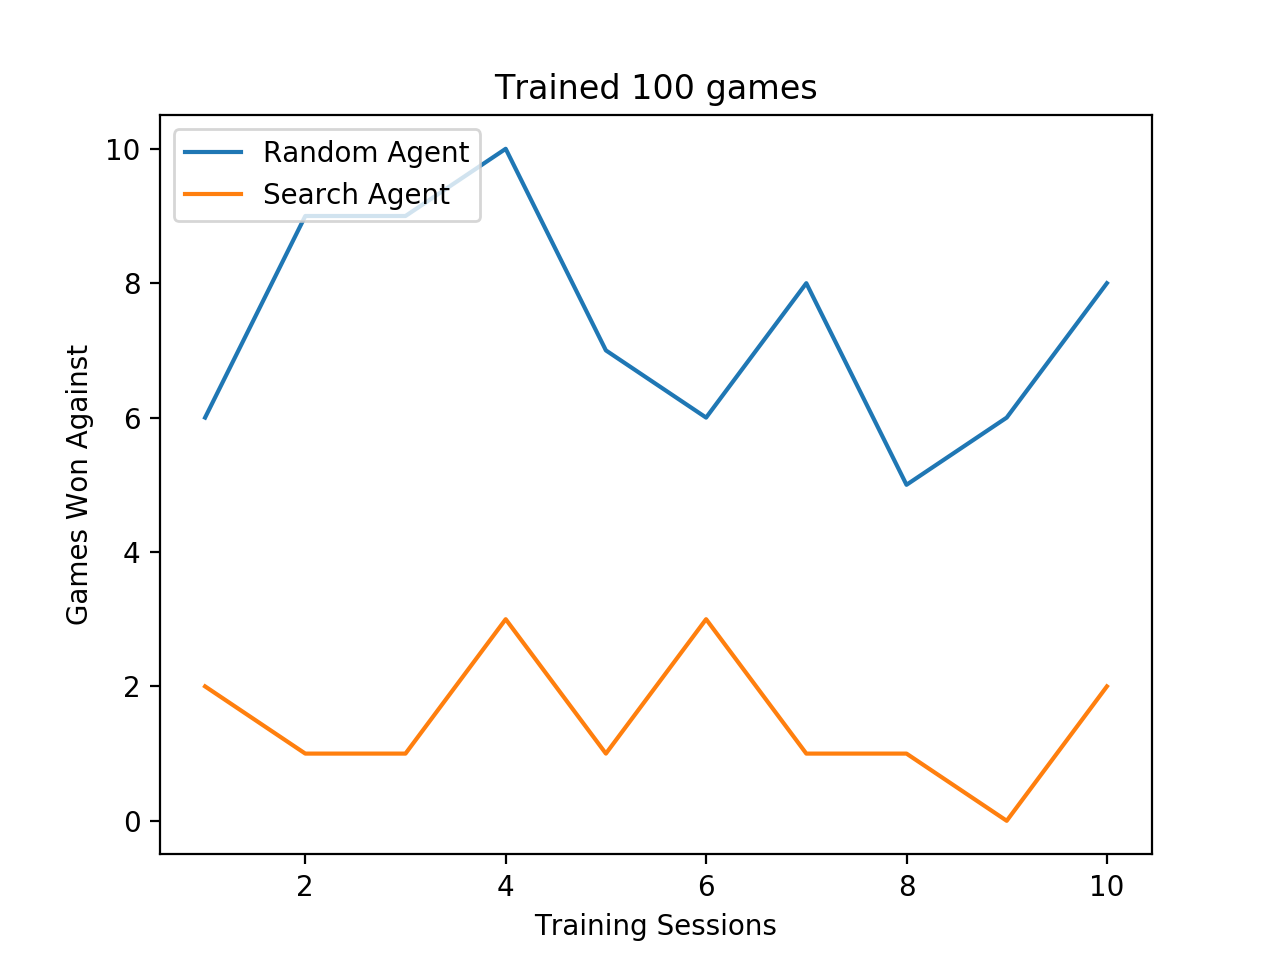
\includegraphics[ width = \columnwidth ]{Assets/100TrainedGames}
	\caption{Our results when sampling over each 100 sessions. What we noted during this was initially increasing behavior against the random agent, which turned into worse behavior as time went on.}
	\label{fig:100TrainedResults}
\end{figure}
\begin{figure}[b]
	\centering
	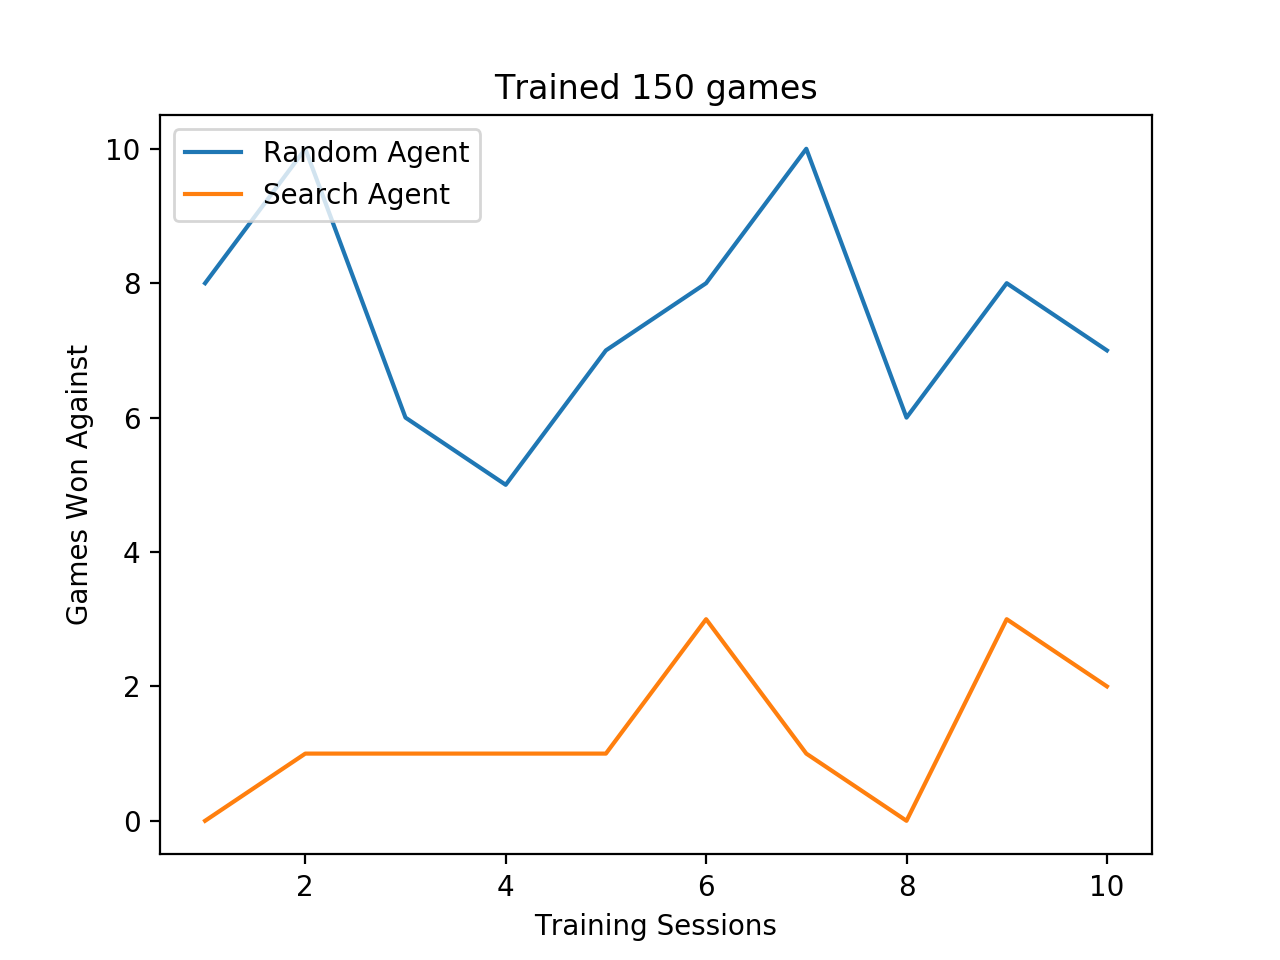
\includegraphics[ width = \columnwidth ]{Assets/150TrainedGames}
	\caption{We noticed a far more erratic behavior for the agent when it was tested after every 150 games. Initially, it performed well, but the sharp decrease came much quicker than in previous cases. When it came to the Search-Based agent, there was far more stable data coming in.}
	\label{fig:150TrainedResults}
\end{figure}
\begin{figure}[b]
	\centering
	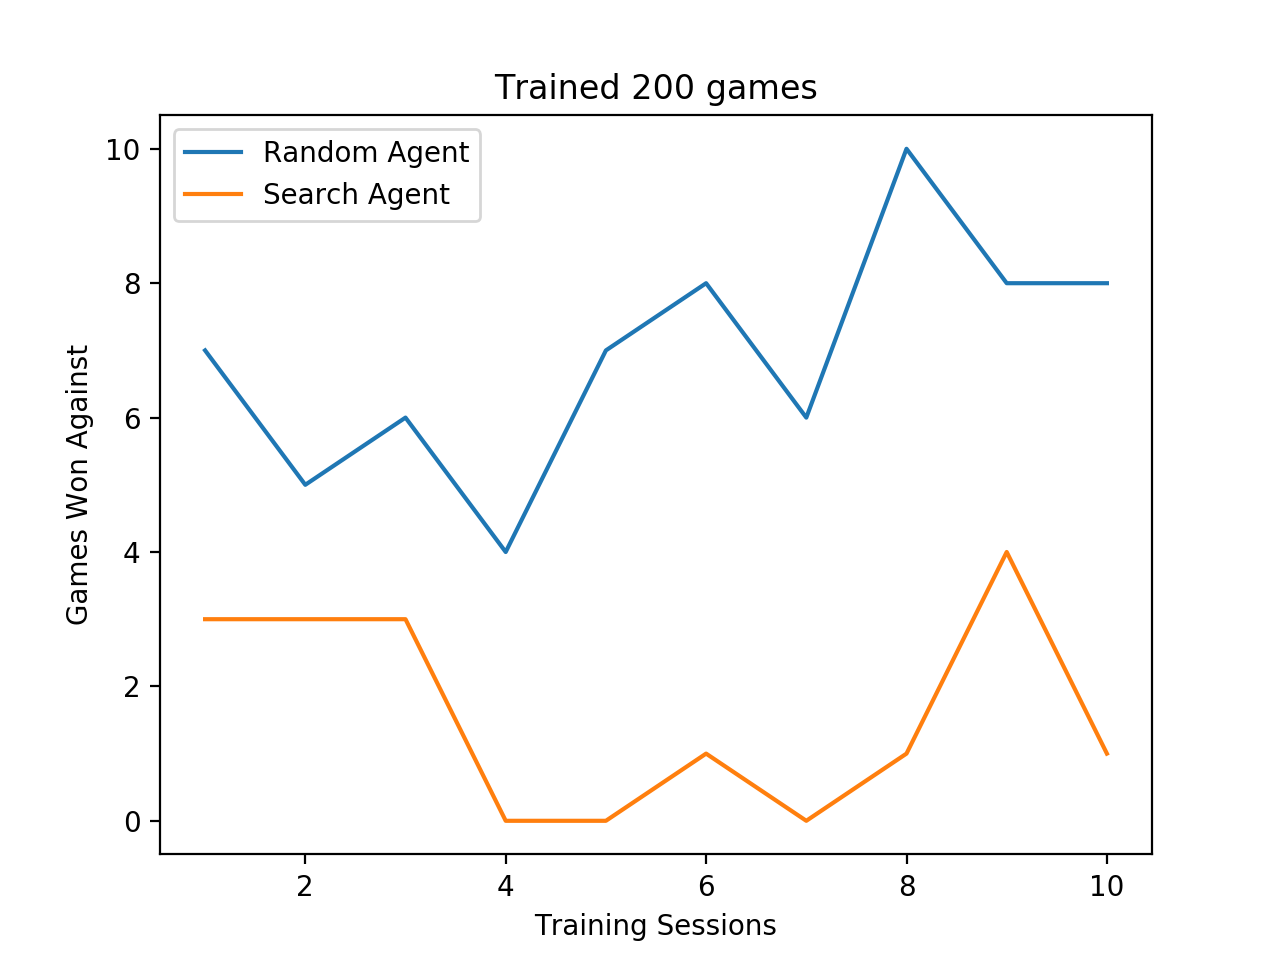
\includegraphics[ width = \columnwidth ]{Assets/200TrainedGames}
	\caption{When it came to 200 training samples before testing, our agent showed an increasing performance against opposing agents. With more computing resources, like the ability to run the code on GPUs, we hope to see that this trend increases as the number of training samples before testing increases.}
	\label{fig:200TrainedResults}
\end{figure}
\begin{figure}[b]
	\centering
	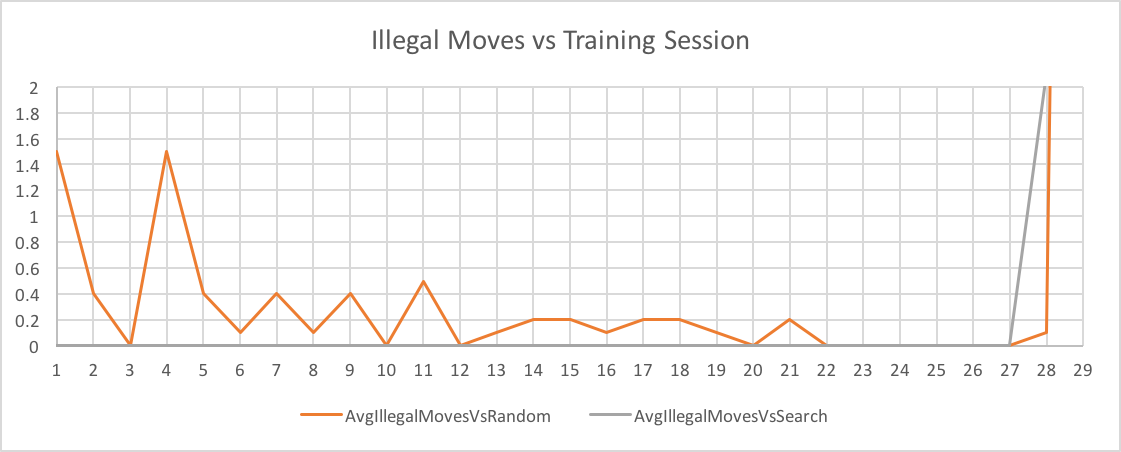
\includegraphics[ width = \columnwidth ]{Assets/pic_png-3}
	\caption{Illegal moves vs training session.  Note how initially the \# of illegal moves is fairly high, then quickly drops to zero.
    Notably, after many training sessions of 0 illegal moves, we observe a spike in the number of illegal moves around training session 28.}
	\label{fig:IllegalMovesTraining}
\end{figure}
\begin{figure}[b]
	\centering
	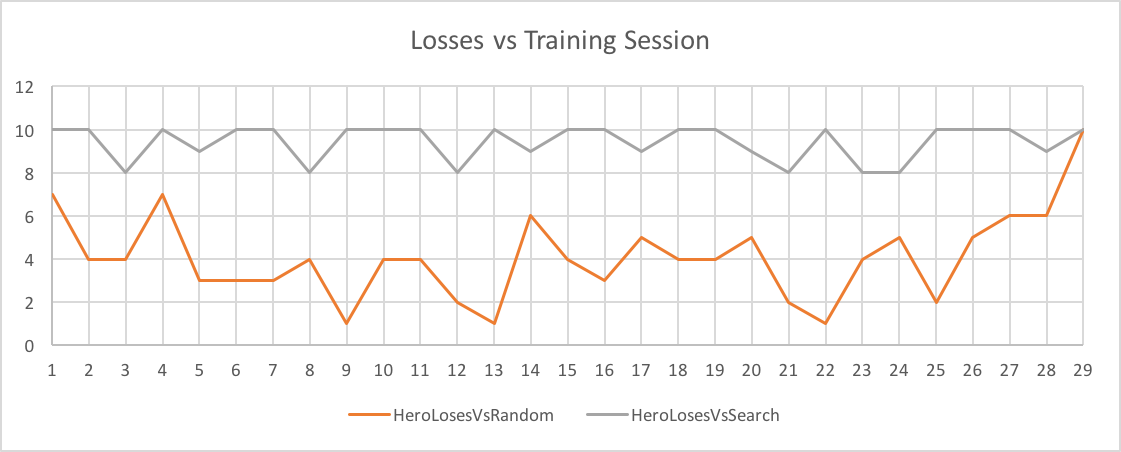
\includegraphics[ width = \columnwidth ]{Assets/pic_png-2}
	\caption{Loss count vs training sessions.
    Note that loss count drops initially, then rises again.
    Particularly, note how sharply the loss count rises as the training session approaches 28.
    We found that with these training sessions, win rate (and illegal moves) really went haywire around training session 28, which indicates noise in the gradient.
   	As described earlier, minibatch-based training is likely the best remedy for this behavior.}
	\label{fig:LossesvTraining}
\end{figure}
\begin{figure}[b]
	\centering
	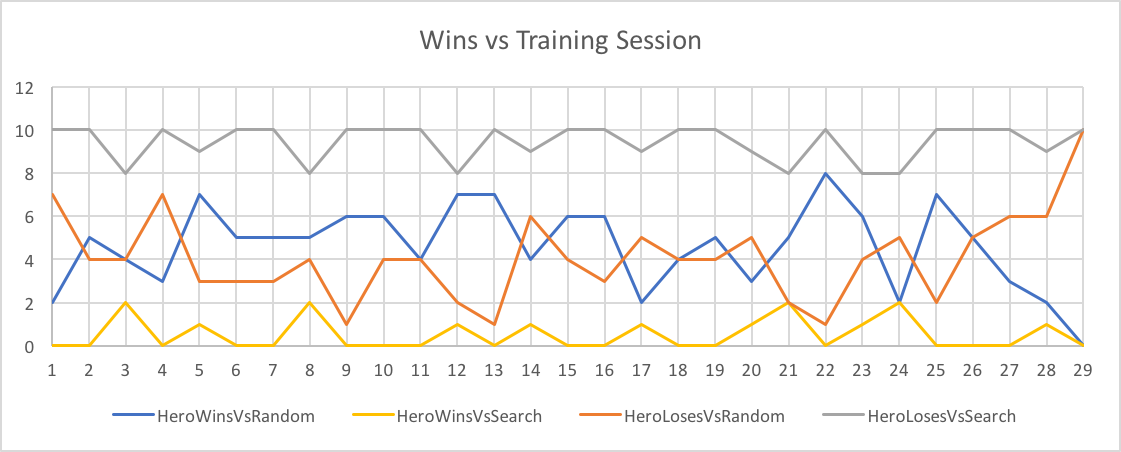
\includegraphics[ width = \columnwidth ]{Assets/pic_png-1}
	\caption{Win (and draw) count vs Training sessions.  Note that wins/losses do not change all that much over the course of training.
    Notably, after the first few training sessions, the maximal (or near it) values for win/draw counts have ben observed}
	\label{fig:WinsvTraining}
\end{figure}




